\documentclass[a4paper,12pt]{article}

\usepackage{amsmath,amssymb,amsthm,tikz}
\usetikzlibrary{calc,arrows.meta}
\usepackage[margin=20mm]{geometry}
\usepackage{fancyvrb}
\usepackage{enumerate}
\usepackage{hyperref}

\setlength{\parindent}{0pt}
\setlength{\columnsep}{1cm}

\begin{document}
\thispagestyle{empty}

\twocolumn

\begin{center}
{\Large Midterm. 2020-10-22},\\
{\em 100 minutes (9:00 \textendash{} 10:40)} 
\end{center}


%(1) Jau gatava C++ koda gabala analīze (tur ir cikli, 
%funkciju izsaukumi - jāatbild uz jautājumiem);
%arī jāuzraksta Big-O notation time complexity tam koda gabalam.
%(2) Objektorientēta C++ koda analīze (virtuālas funkcijas: 
%Jāpasaka, kura funkcija tiks izsaukta - vecāka klasē vai bērna klasē). 
%Ja kāds fiksi mācēs testēt kodu - varēs pārbaudīt uz sava kompilatora; 
%bet bez izpratnes cilvēki ar šo var kļūdīties.
%(3) Daži piemēri par Big-O notation - jāsalīdzina funkciju augšana.  
%(4) Stekam dots pseidokods, kur ar "push()" un "pop()" kaut ko dara; 
%jāuzraksta steka stāvokļi pēc komandu izpildes.
%(5) Uzdevums, kurā noteiktā veidā jāapstaigā pilns/complete koks, 
%kas dots ar masīvu (post-order, piemēram). Visnotaļ līdzīgs tam piemēram, 
%kuru atsūtīji - iespējams, mazliet vienkāršāks 
%(koks ir pilns - tātad tukšu vietu masīvā nemaz nav)



\vspace{10pt}
{\bf Question 1.} 

There is a 2-dimensional array $\mathtt{arr}$ 
of size $n$ by $n$; its elements are
integer numbers (each number contains no more than $n$ digits in 
its decimal representation). 

You are given this C++ code with function {\tt main()} calling function {\tt fun()}.
%On Line ? of this code we perform {\em integer division} (for example, $7/2$ equals $3$). 


{\footnotesize
\begin{center}
\begin{minipage}{.85\columnwidth}
\begin{Verbatim}[frame=single,numbers=left]
int fun(int row) {
  int count = 0;
  for (int col=0; col<n; col++) {
    while (arr[row][col]>0) {
      arr[row][col] /= 2;
      count++;
    }
  }
  return count;
}


int main() {
  for (int row=0; row<n; row++) {
    cout << fun(row);
  }
}
\end{Verbatim}
\end{minipage}
\end{center}
}

Analyze the time complexity of this algorithm 
``inside out'':

\begin{enumerate}[(A)]
\item Estimate with some $O(g(n))$ the time spent 
on a single iteration of the loop in 
Lines 5-6. (How fast one can run these lines
just once.)
\item Estimate with some $O(g(n))$ the time spent
on the loop Lines 4-7 (for one specific pair 
of row,col). 
\item Estimate with some $O(g(n))$ the 
time spent in the outer loop on Lines 3-8. 
(And also in a single call of {\tt fun(...)}.)
\item Estimate the time spent in the loop 
on Lines 14-16. 
\end{enumerate}


\textcolor{blue}{\footnotesize
{\em Note.} We use integer division in this algorithm; 
for example {\tt 7/2} equals {\tt 3} and {\tt 1/2} equals {\tt 0}. So it will eventually stop.
}






\vspace{20pt}
{\bf Question 2.} 

Definition of Big-O:\\
Real-valued function with natural arguments $f(n)$ is in 
$O(g(n))$ iff there exist $C,n_0 >0$ such that
$$|f(n)| \leq C \cdot |g(n)|,$$
whenever $n > n_0$. 

\begin{enumerate}[(A)]
\item Use the definition of Big-O Notation to 
prove or to disprove that $f(n) = 100n^2 + \frac{1}{4}n^3$
is in $O(n^3)$. 
\item Use the definition of Big-O Notation to 
prove or to disprove that $f(n) = (\log_2 n)^2$
is in $O(\log_2 n)$. 
\end{enumerate}

The reasoning should either provide the examples of $C,n_0$ 
that satisfy the definition for any $n$; or a method that 
for any given $C,n_0$ finds find $n$ such that the definition is not satisfied.




\vspace{20pt}
{\bf Question 3.} 

Consider the Queue implementation from \url{https://bit.ly/35n7bKd}.

Denote $a,b,c$ to be the last $3$ digits of your Student ID, and compute the following numbers: 
\begin{itemize}
\item $F = ((a+b+c)\;\operatorname{mod}\;3) + 2$
\item $\mathtt{x1} = (a+b+c)\;\operatorname{mod}\;10$
\item $\mathtt{x2} = ((a+b) \cdot 2)\;\operatorname{mod}\;10$
\item $\mathtt{x3} = ((b+c) \cdot 3)\;\operatorname{mod}\;10$
\item $\mathtt{x4} = ((c+a) \cdot 7)\;\operatorname{mod}\;10$
\end{itemize}

The queue $Q$ is implemented as an array of size $N=6$; its elements
have indices from $\{0,1,2,3,4,5\}$. 

Initially the queue parameters are these:\\
$\mathtt{Q.front} = \mathtt{F}$,\\
$\mathtt{Q.length} = 4$,\\
$\mathtt{Q.size} = 6$.\\
And the content of the array is the following:

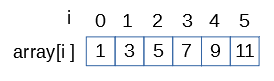
\includegraphics[width=2in]{midterm/midterm-queue-structure.png}

Somebody runs the following code on this queue:

\begin{verbatim}
Q.enqueue(x1)
Q.enqueue(x2)
Q.dequeue()
Q.dequeue()
// show the state of Q
Q.enqueue(x3)
Q.enqueue(x4)
Q.dequeue()
// show the state of Q
\end{verbatim}

After Line 4 (and at the very end) show the current state of the queue $\mathtt{Q}$. 
The state should display the content of the array and also the values of 
$\mathtt{Q.front}$ and $\mathtt{Q.length}$. 

You can use shading, if it helps to visualize the array cells that are not 
currently used by your queue.


\textcolor{blue}{\footnotesize
{\em Note.} Painting something gray is not required (since front/length indicate the state of your queue anyway). But painting cells gray may be helpful, if you want to visualize where your queue has the useful values (and what is some old garbage \textendash{} you can shade it over).
}


% https://www.geeksforgeeks.org/iterative-postorder-traversal-using-stack/
\vspace{20pt}
{\bf Question 4.} 

{\footnotesize
{\bf Introduction.} 
Binary trees are often represented as arrays 
(where the array starts with the root node; followed
by all the other nodes, displayed layer by layer. 
If any child of a node in this tree is missing, it is replaced by 
$\Lambda$ (capital Lambda denoting an empty tree)
in the array. Once we reach the last non-empty node in the tree, this is
the last element of the array. 
For example, the binary tree shown in this picture:

\begin{figure}[!htb]
\center{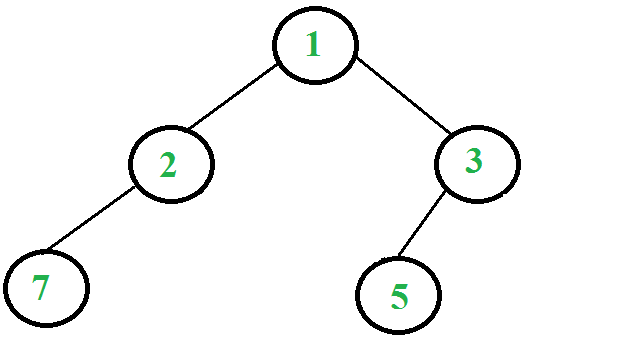
\includegraphics[width=2in]{midterm/example-binary-tree.png}}
\caption{\label{fig:example-binary-tree} Example binary tree.}
\end{figure}
is represented by the following array: 
$$\mathtt{int\;a[\,]\;=\;\{1,2,3,7,\Lambda,5\}};$$

}

\vspace{10pt}
{\bf Problem.} 
Assume that you have a binary tree that is represented by the following array:
\textcolor{red}{
\begin{equation}
\label{eq:treearr}
\mathtt{int\;a[\,]\;=\;\{1, 2, 4, a, \Lambda, \Lambda, 6, b, \Lambda, \Lambda, \Lambda, \Lambda, \Lambda, \Lambda, c\};}
\end{equation}
}

Values $a$, $b$, $c$ are the last three digits taken from your Student ID.\\
\textcolor{blue}{\footnotesize
{\em Note.} In the original the array contained a mistake (it had four $\Lambda$ 
instead of six; but this was wrong, it does not correspond to any tree). 
}


\begin{enumerate}[(A)]
\item Draw the binary tree represented by the array \ref{eq:treearr} in your answer. 
The tree should look nice: 
Draw left children to the left (and right children to the right)
of their parents. Nodes on the same levels should be aligned. 
\item What is the number of internal nodes in this tree? The number of leaves in this tree?
\item List the vertices of this tree in the post-order traversal order.\\
\textcolor{blue}{\footnotesize
{\em Note.} You only show real nodes in the post-order sequence (all $\Lambda$ are 
just technical symbols indicating absence of nodes; they are not part of the tree). 
}
\item Write pseudo-code for an algorithm\\ 
$\text{\textsc{getParent}}(i)$ that receives 
the index $i$ of some node in this array, returns the index of the parent of this node (or $-1$, if the node has no parent). 
All indices $i$ are zero-based (in an array of length $10$, $i \in \{0,\ldots,9\}$).
\item Assume that there is a different array (representing another binary tree) which does not contain any $\Lambda$ 
values; all values there represent some nodes. Describe the property such trees must satisfy.  
\end{enumerate}




\end{document}



